% Options for packages loaded elsewhere
\PassOptionsToPackage{unicode}{hyperref}
\PassOptionsToPackage{hyphens}{url}
\PassOptionsToPackage{dvipsnames,svgnames,x11names}{xcolor}
\documentclass[
  11pt,
  a4paper,
]{article}
\usepackage{xcolor}
\usepackage[margin=24mm]{geometry}
\usepackage{amsmath,amssymb}
\setcounter{secnumdepth}{5}
\usepackage{iftex}
\ifPDFTeX
  \usepackage[T1]{fontenc}
  \usepackage[utf8]{inputenc}
  \usepackage{textcomp} % provide euro and other symbols
\else % if luatex or xetex
  \usepackage{unicode-math} % this also loads fontspec
  \defaultfontfeatures{Scale=MatchLowercase}
  \defaultfontfeatures[\rmfamily]{Ligatures=TeX,Scale=1}
\fi
\usepackage{lmodern}
\ifPDFTeX\else
  % xetex/luatex font selection
\fi
% Use upquote if available, for straight quotes in verbatim environments
\IfFileExists{upquote.sty}{\usepackage{upquote}}{}
\IfFileExists{microtype.sty}{% use microtype if available
  \usepackage[]{microtype}
  \UseMicrotypeSet[protrusion]{basicmath} % disable protrusion for tt fonts
}{}
\makeatletter
\@ifundefined{KOMAClassName}{% if non-KOMA class
  \IfFileExists{parskip.sty}{%
    \usepackage{parskip}
  }{% else
    \setlength{\parindent}{0pt}
    \setlength{\parskip}{6pt plus 2pt minus 1pt}}
}{% if KOMA class
  \KOMAoptions{parskip=half}}
\makeatother
\usepackage{longtable,booktabs,array}
\newcounter{none} % for unnumbered tables
\usepackage{calc} % for calculating minipage widths
% Correct order of tables after \paragraph or \subparagraph
\usepackage{etoolbox}
\makeatletter
\patchcmd\longtable{\par}{\if@noskipsec\mbox{}\fi\par}{}{}
\makeatother
% Allow footnotes in longtable head/foot
\IfFileExists{footnotehyper.sty}{\usepackage{footnotehyper}}{\usepackage{footnote}}
\makesavenoteenv{longtable}
\usepackage{graphicx}
\makeatletter
\newsavebox\pandoc@box
\newcommand*\pandocbounded[1]{% scales image to fit in text height/width
  \sbox\pandoc@box{#1}%
  \Gscale@div\@tempa{\textheight}{\dimexpr\ht\pandoc@box+\dp\pandoc@box\relax}%
  \Gscale@div\@tempb{\linewidth}{\wd\pandoc@box}%
  \ifdim\@tempb\p@<\@tempa\p@\let\@tempa\@tempb\fi% select the smaller of both
  \ifdim\@tempa\p@<\p@\scalebox{\@tempa}{\usebox\pandoc@box}%
  \else\usebox{\pandoc@box}%
  \fi%
}
% Set default figure placement to htbp
\def\fps@figure{htbp}
\makeatother
\setlength{\emergencystretch}{3em} % prevent overfull lines
\providecommand{\tightlist}{%
  \setlength{\itemsep}{0pt}\setlength{\parskip}{0pt}}
% Shared style; used by generated, standalone LaTeX sources.
\usepackage{xcolor}
\usepackage{xurl}
\usepackage{fvextra}
\usepackage{etoolbox}
\usepackage{fancyhdr}
\usepackage{titlesec}
\definecolor{researchblue}{HTML}{173B58}
\AtBeginDocument{\hypersetup{linkcolor=researchblue,urlcolor=researchblue}}
\pagestyle{fancy}
\fancyhf{}
\fancyhead[L]{\small\sffamily SVG PATCH LAB}
\fancyhead[R]{\small\sffamily CVPR 2027 research package}
\fancyfoot[L]{\small Working documents; results and proposals distinguished}
\fancyfoot[R]{\thepage}
\setlength{\headheight}{15pt}
\setlength{\emergencystretch}{3em}
\titleformat{\section}{\Large\bfseries\color{researchblue}}{\thesection}{0.7em}{}
\titleformat{\subsection}{\large\bfseries\color{researchblue}}{\thesubsection}{0.7em}{}
\DefineVerbatimEnvironment{verbatim}{Verbatim}{breaklines=true,breakanywhere=true,fontsize=\small}
\AtBeginEnvironment{longtable}{\small\setlength{\tabcolsep}{4pt}}
\let\originaltableofcontents\tableofcontents
\renewcommand{\tableofcontents}{\originaltableofcontents\clearpage}
\usepackage{bookmark}
\IfFileExists{xurl.sty}{\usepackage{xurl}}{} % add URL line breaks if available
\urlstyle{same}
\hypersetup{
  pdftitle={Completed Results and Failure Audit},
  pdfauthor={SVG Patch Lab - Research Working Package},
  colorlinks=true,
  linkcolor={Maroon},
  filecolor={Maroon},
  citecolor={Blue},
  urlcolor={blue},
  pdfcreator={LaTeX via pandoc}}

\title{Completed Results and Failure Audit}
\author{SVG Patch Lab - Research Working Package}
\date{14 September 2026 \textbar{} CVPR 2027 target}

\begin{document}
\maketitle

{
\setcounter{tocdepth}{2}
\tableofcontents
}
13 September 2026. \textbf{The earlier report overstated the evidence
for three general classes of Astra failure.} The historical Robin case
did exhaust its token budget, but both new calls returned accurate
contours under the present sampled metric. The capacitor's alleged
closed field loops are not present in its saved paths. The bracket
output explicitly discloses that its stress colors are illustrative
rather than a solved FEM field.

This report supersedes the strong qualitative failure claims in the
older overview/proposal. Original files remain intact for provenance. It
does not assert that Astra reliably solves arbitrary FEM problems.

\section{Direct OpenAI API reruns}\label{direct-openai-api-reruns}

The existing local credential was verified against the direct OpenAI
model endpoint. Calls used \texttt{gpt-6-astra}, the original task texts
and generation wrapper, Chat Completions, \texttt{store=false}, and one
sample per condition. No key is copied into these artifacts. Model
access and parameters were checked against
\href{https://developers.openai.com/api/docs/models/gpt-6-astra}{official
Astra documentation}.

{\def\LTcaptype{none} % do not increment counter
\begin{longtable}[]{@{}
  >{\raggedright\arraybackslash}p{(\linewidth - 8\tabcolsep) * \real{0.1765}}
  >{\raggedright\arraybackslash}p{(\linewidth - 8\tabcolsep) * \real{0.1765}}
  >{\raggedright\arraybackslash}p{(\linewidth - 8\tabcolsep) * \real{0.1765}}
  >{\raggedleft\arraybackslash}p{(\linewidth - 8\tabcolsep) * \real{0.2353}}
  >{\raggedleft\arraybackslash}p{(\linewidth - 8\tabcolsep) * \real{0.2353}}@{}}
\toprule\noalign{}
\begin{minipage}[b]{\linewidth}\raggedright
Case
\end{minipage} & \begin{minipage}[b]{\linewidth}\raggedright
Effort / token cap
\end{minipage} & \begin{minipage}[b]{\linewidth}\raggedright
Finish
\end{minipage} & \begin{minipage}[b]{\linewidth}\raggedleft
Completion / reasoning tokens
\end{minipage} & \begin{minipage}[b]{\linewidth}\raggedleft
Wall time
\end{minipage} \\
\midrule\noalign{}
\endhead
\bottomrule\noalign{}
\endlastfoot
Convective plate & medium / 16,000 & stop, SVG & 15,329 / 11,775 &
297.90 s \\
Convective plate & medium / 32,000 & stop, SVG & 17,697 / 14,660 &
334.30 s \\
Finite capacitor & low / 16,000 & stop, SVG & 3,120 / 512 & 48.83 s \\
L-bracket stress & low / 16,000 & stop, SVG & 3,439 / 512 & 63.23 s \\
\end{longtable}
}

All four attempts, request payloads, response IDs, full responses and
usage are retained in \nolinkurl{runs/astra-api-recheck-20260913/}. The
protocol was saved before calls. Total usage was 1,312 input and 39,585
completion tokens, approximately \textbf{\$1.99} at the documented
standard \$10/\$50 per million input/output tokens; this is a
token-price estimate, not an invoice.
\href{https://developers.openai.com/api/docs/models/gpt-6-astra}{Pricing
source}.

The paired Robin conditions change the budget only. One sample each
cannot isolate a budget effect statistically. A historical model alias
may also resolve differently over time; no failure-rate or model-wide
capability claim follows from these four calls.

\section{Robin heat conduction: historical truncation, not
reproduced}\label{robin-heat-conduction-historical-truncation-not-reproduced}

The original \texttt{plate\_convective\_edges} record contains 16,000
completion tokens, all reported as reasoning,
\texttt{finish\_reason=length}, and no SVG. This is a real completion
failure for that call. It is not enough to conclude that Robin
boundaries are beyond the model's capability.

The independent reference solves \(\nabla\)\(^2\)T=0 on {[}0,2{]}
\(\times\) {[}0,1{]}, with T=100 °C on the left, ambient 0 °C and
outward derivative \(\partial\)T/\(\partial\)n=-5T on the other three
edges. The P2 Galerkin weak form adds the Robin boundary integral
\texttt{integral\ 5\ T\ v} to the stiffness form. Implementation uses
\href{https://scikit-fem.readthedocs.io/en/stable/api.html}{scikit-fem
boundary forms}.

Reference checks include an exact linear Robin anchor, discrete heat
balance and five meshes from 576 to 147,456 triangles. The finest mesh
has 296,065 degrees of freedom. The last two meshes differ by at most
0.02053 °C on the common regular grid, and by at most 0.00797 °C at the
sampled model-contour points. These differences estimate numerical
sensitivity; they are not certified continuum error bounds. The old
first-order finite-difference reference differs from the fine FEM grid
by up to 1.977 °C, so it should not be treated as exact ground truth.

The primary recheck evaluates temperature \textbf{directly in the FEM
basis} along the transformed SVG paths, at maximum physical sampling
step 0.002. The five required levels are present and no unsupported
contour features were flagged.

{\def\LTcaptype{none} % do not increment counter
\begin{longtable}[]{@{}
  >{\raggedright\arraybackslash}p{(\linewidth - 6\tabcolsep) * \real{0.2143}}
  >{\raggedleft\arraybackslash}p{(\linewidth - 6\tabcolsep) * \real{0.2857}}
  >{\raggedleft\arraybackslash}p{(\linewidth - 6\tabcolsep) * \real{0.2857}}
  >{\raggedright\arraybackslash}p{(\linewidth - 6\tabcolsep) * \real{0.2143}}@{}}
\toprule\noalign{}
\begin{minipage}[b]{\linewidth}\raggedright
New response
\end{minipage} & \begin{minipage}[b]{\linewidth}\raggedleft
Arc-length-weighted mean error
\end{minipage} & \begin{minipage}[b]{\linewidth}\raggedleft
Maximum sampled error
\end{minipage} & \begin{minipage}[b]{\linewidth}\raggedright
Pass at 0.5 °C
\end{minipage} \\
\midrule\noalign{}
\endhead
\bottomrule\noalign{}
\endlastfoot
16,000-token cap & 0.00702 °C & 0.11074 °C & Yes \\
32,000-token cap & 0.01247 °C & 0.37385 °C & Yes \\
\end{longtable}
}

The separately retained regular-grid audit gives slightly larger maxima,
0.12698 and 0.38381 °C, because it adds interpolation error. Use the
direct FEM scores above for the primary numerical comparison. Larger
token budget did not improve the measured error in this pair; neither a
benefit nor a disadvantage is established with one call per condition.

\begin{figure}
\centering
\pandocbounded{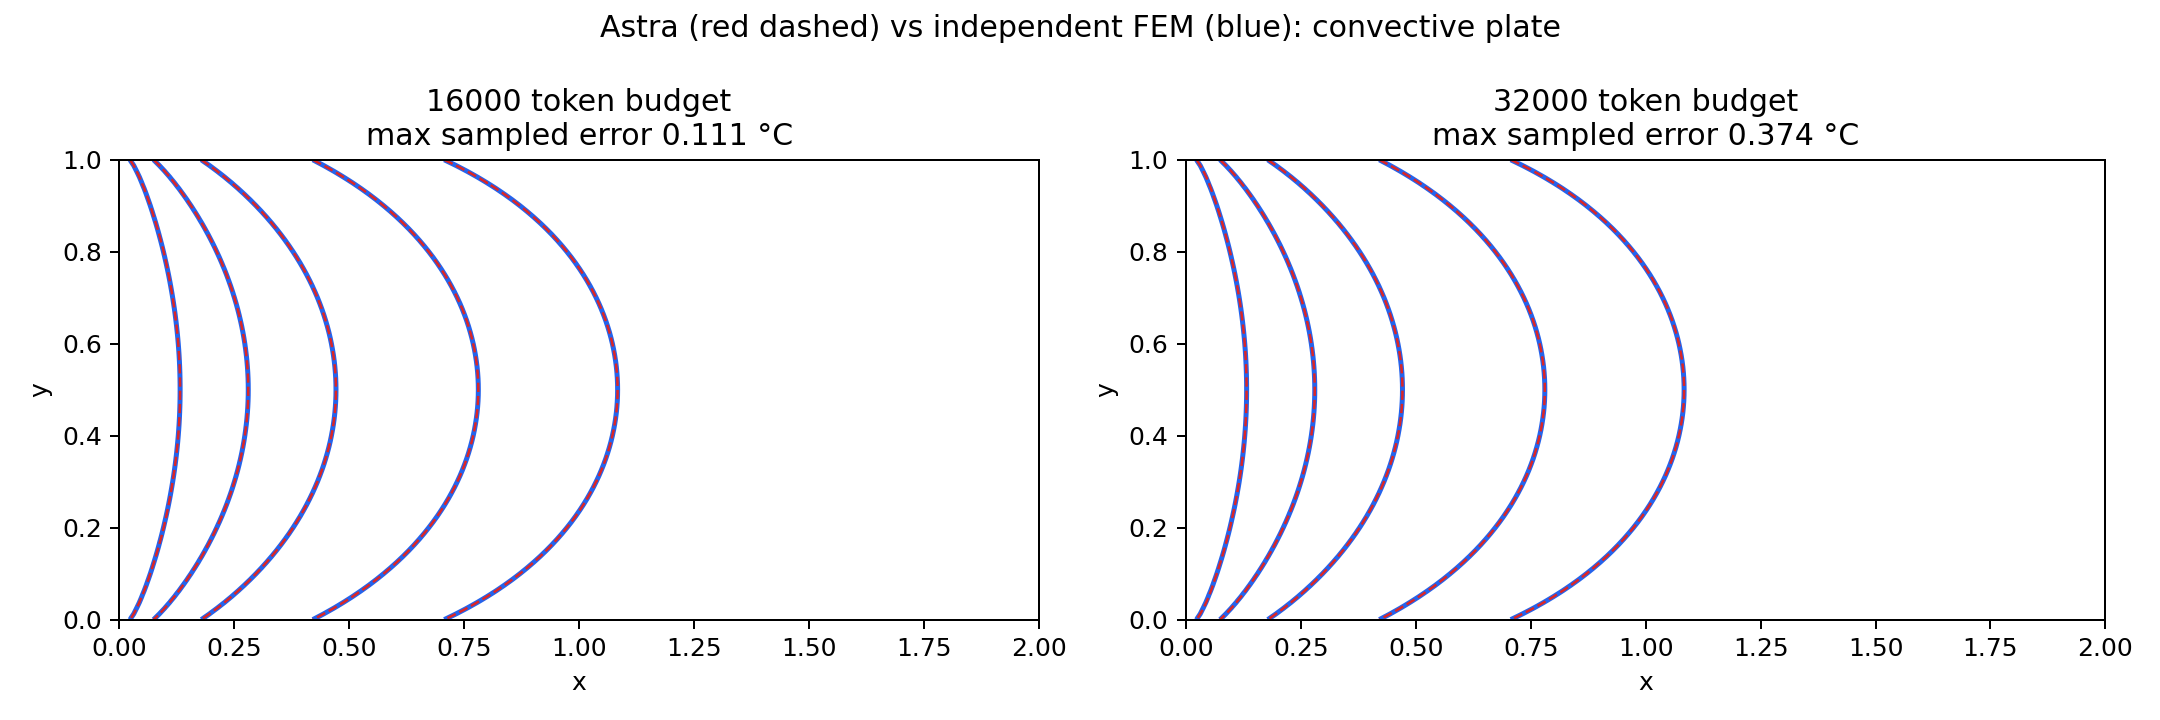
\includegraphics[keepaspectratio,alt={Astra contours compared with FEM}]{../../runs/astra-api-recheck-20260913/robin_fem_comparison.png}}
\caption{Astra contours compared with FEM}
\end{figure}

These are geometric contour checks. They do not certify all rendered
labels, occlusion, units, or the boundary-angle condition separately.
Numerical agreement along samples is not a mathematical certificate.

\section{Capacitor: retract the closed-loop
claim}\label{capacitor-retract-the-closed-loop-claim}

The historical artifact has 12 selected electric-field paths,
\textbf{zero closed paths}, and every selected path joins the positive
and negative plate. The source explicitly includes ``End contours
schematic.'' The apparent circular lobes in the figure are open paths
terminating on conductors. Its open equipotential endpoints also do not
by themselves establish behavior at infinity.

A source-specific path-intersection diagnostic finds a maximum departure
from perpendicularity of about 8.04 degrees at computed
field/equipotential intersections, with no failed intersection pairs.
This supports describing the rendering as approximate. It does not
establish that the field is physically impossible, nor is it a
substitute for an electrostatic solve. The new response again labels its
end fringing as schematic.

Needed for a fair quantitative test: specify whether this is a 2-D
cross-section or a 3-D finite plate, conductor thickness/width, the
exterior/far-boundary treatment, and the field quantity to evaluate.
Then use a converged FEM/BEM or independent electrostatic reference.
Until then, numerical fidelity is \textbf{unverified}, not a
demonstrated closed-loop failure.

Evidence:
\nolinkurl{runs/astra-historical-audit/capacitor_geometry.json};
reproducible source-specific checker:
\nolinkurl{scripts/audit_historical_capacitor.py}.

\section{Bracket: disclosed approximation and under-specified peak
stress}\label{bracket-disclosed-approximation-and-under-specified-peak-stress}

Both historical and fresh outputs give the approximately 122 MPa
beam-theory nominal stress under the stated interpretation of 80 mm
out-of-plane width, 8 mm thickness and 52 mm lever arm. Both illustrate
a roughly 220 MPa hotspot using an assumed factor near 1.8 and disclose
that this is not a solved FEM result.

The fresh SVG states that a finite peak requires a fillet radius,
bolt/contact assumptions and a converged mesh. The original prompt asks
for an expected field and estimated peak without specifying these
inputs. Scoring the illustration as a numerically solved von Mises field
would misrepresent both the prompt and the response. The legitimate gap
is that the picture does not supply a solved, verifiable stress field.

A next test should prescribe complete geometry, plane-stress/3-D
assumptions, material law, support/contact conditions, load distribution
and fillet. Compare displacement, reactions and stress away from
singular boundaries, then perform a convergence study for any peak
claim. Reusing the infinite-plate Kirsch factor as exact truth for a
finite square plate is also invalid; the earlier local FEM smoke results
already show a finite-domain difference.

\section{What the project needs to
address}\label{what-the-project-needs-to-address}

\begin{enumerate}
\def\labelenumi{\arabic{enumi}.}
\tightlist
\item
  \textbf{Completion reliability:} retain token use and empty/truncated
  attempts, with repeated cases and budgets. A single failure cannot
  define a PDE-class limit.
\item
  \textbf{Numerical reference quality:} mesh convergence, analytic
  anchors, physical balance and direct field evaluation before labeling
  model error.
\item
  \textbf{Honest claim status:} distinguish an approximation, a solved
  field, a verified geometry and a fully reviewed drawing. Treat
  disclosed approximations differently from undisclosed numerical
  claims.
\item
  \textbf{Physical edits:} rerun FEM when loads, material, geometry or
  boundary conditions change, then update the visible field, quantity,
  units and labels together.
\item
  \textbf{Stronger evaluation:} well-posed finite elasticity,
  multiphysics and sequential visual edits with repeated samples and
  independent references. The current evidence does not justify saying
  Astra generally fails at FEM.
\end{enumerate}

The \href{../../reports/FEM_LITERATURE_AND_EXTENSION.md}{FEM literature
survey} identifies the existing simulation and training systems to build
on. The new FEM-Bench bridge performs actual solver reruns; the earlier
Qwen action-policy training is retained as a separate infrastructure
pilot.

Reproduction from \texttt{cvpr2027/}:

\begin{verbatim}
PYTHONPATH=src ../.venv/bin/python scripts/robin_fem_reference.py --output runs/robin-fem-reference --fd-reference runs/reference-v3/plate_convective_edges.npz
PYTHONPATH=src ../.venv/bin/python scripts/score_astra_robin_fem.py --runs runs/astra-api-recheck-20260913 --reference runs/robin-fem-reference
../.venv/bin/python scripts/fem_bench_svg_extension.py --output runs/fem-bench-svg-anchor
\end{verbatim}

\clearpage

\section{A100 training results}\label{a100-training-results}

Three Qwen2.5-Coder-1.5B-Instruct LoRA runs completed on an NVIDIA
A100-SXM4-40GB: seeds 17, 29 and 41, three full epochs and 90 optimizer
steps each. Adapter weights, final/previous optimizer checkpoints, exact
data, raw predictions, package versions and source hashes are saved
locally in \texttt{runs/a100/}. Final adapters, predictions and
manifests are versioned in this branch; intermediate optimizer
checkpoints and ZIP downloads remain local ignored files. The original
downloaded archive is \texttt{runs/a100-completed.zip} (350,830,393
bytes).

\texttt{scripts/summarize\_training.py} verified completion, data and
source hashes, case-disjoint splits, all 720 raw base/final predictions,
and the three safetensors adapter structures. Each adapter contains
4,358,144 parameters. Model revision:
\nolinkurl{2e1fd397ee46e1388853d2af2c993145b0f1098a}. The separate
saved-adapter inference reload check was prepared but was \textbf{not
run} before Colab disconnected; no reload result is claimed.

{\def\LTcaptype{none} % do not increment counter
\begin{longtable}[]{@{}
  >{\raggedright\arraybackslash}p{(\linewidth - 8\tabcolsep) * \real{0.1579}}
  >{\raggedleft\arraybackslash}p{(\linewidth - 8\tabcolsep) * \real{0.2105}}
  >{\raggedleft\arraybackslash}p{(\linewidth - 8\tabcolsep) * \real{0.2105}}
  >{\raggedleft\arraybackslash}p{(\linewidth - 8\tabcolsep) * \real{0.2105}}
  >{\raggedleft\arraybackslash}p{(\linewidth - 8\tabcolsep) * \real{0.2105}}@{}}
\toprule\noalign{}
\begin{minipage}[b]{\linewidth}\raggedright
Model / policy
\end{minipage} & \begin{minipage}[b]{\linewidth}\raggedleft
Test strict exact action
\end{minipage} & \begin{minipage}[b]{\linewidth}\raggedleft
Annulus strict exact action
\end{minipage} & \begin{minipage}[b]{\linewidth}\raggedleft
Test fence-normalized
\end{minipage} & \begin{minipage}[b]{\linewidth}\raggedleft
Annulus fence-normalized
\end{minipage} \\
\midrule\noalign{}
\endhead
\bottomrule\noalign{}
\endlastfoot
Base Qwen, each seed & 0/60 & 0/60 & 26/60 & 25/60 \\
Final LoRA, seed 17 & 60/60 & 60/60 & 60/60 & 60/60 \\
Final LoRA, seed 29 & 60/60 & 60/60 & 60/60 & 60/60 \\
Final LoRA, seed 41 & 60/60 & 60/60 & 60/60 & 60/60 \\
Deterministic template parser & 60/60 & 60/60 & 60/60 & 60/60 \\
\end{longtable}
}

Training plus adapter-save times were 94.94, 98.61 and 99.42 seconds
respectively; these exclude base/final evaluation and environment/model
setup. The live notebook and logs retain the complete execution record.
No cost estimate is inferred from these timings.

The strict base score is heavily affected by Markdown JSON fences. The
separate normalization measure removes only one enclosing fence; it does
not choose a convenient object from malformed or multiple-object
responses. The base also makes action errors, so normalization does not
make it perfect.

This is a compact-DOM, shared-template action policy, not a trained FEM
solver or vision model. Each evaluation split contains only ten
independent physical cases, with six edits each. Repeated seeds do not
increase the number of independent test cases. The perfect rule baseline
makes the result pipeline validation, not evidence that learning is
needed. The next engineering study is described in the
\href{../../reports/FEM_LITERATURE_AND_EXTENSION.md}{FEM literature and
extension report}.

\section{Provenance and recovery}\label{provenance-and-recovery}

An initial three-seed A100 run finished but lost its temporary weights
before download. Its notebook/console logs are preserved as
\texttt{runs/a100-first-run-*}; those logs are not counted as three
additional independent experiments. The recovery run repeated the same
configuration and downloaded automatically on completion. The verified
results above refer only to the recovered, locally saved artifacts. An
earlier T4 attempt was interrupted and is retained separately.

The GPU-generated JSONL bytes differ from the original local data
because numerical-library serialization differs. Every model input and
target matches the local splits; all three GPU runs have identical split
hashes. Use the exact data inside each GPU run to reproduce hashes and
executor scoring.

Recheck from \texttt{cvpr2027/}:

\begin{verbatim}
../.venv/bin/python scripts/summarize_training.py --runs runs/a100 --output reports/training_verified.json
\end{verbatim}

Machine-readable evidence: \nolinkurl{reports/training_verified.json}.
Completed notebook: \nolinkurl{notebooks/A100_completed_runs.ipynb}. The
Colab runtime is disconnected; no GPU training remains active.

\section{Historical audit and manufactured
controls}\label{historical-audit-and-manufactured-controls}

Earlier proposal PDFs and TeX files predate the evaluator repair. Their
claims of universally validated contour fidelity and their preliminary
success totals must \textbf{not} be copied into a submission without
re-audit. Historical files remain intact for provenance.

At a maximum sampled error threshold of 0.5 percentage points of the
specified field range:

{\def\LTcaptype{none} % do not increment counter
\begin{longtable}[]{@{}
  >{\raggedright\arraybackslash}p{(\linewidth - 8\tabcolsep) * \real{0.1667}}
  >{\raggedleft\arraybackslash}p{(\linewidth - 8\tabcolsep) * \real{0.2222}}
  >{\raggedleft\arraybackslash}p{(\linewidth - 8\tabcolsep) * \real{0.2222}}
  >{\raggedleft\arraybackslash}p{(\linewidth - 8\tabcolsep) * \real{0.2222}}
  >{\raggedright\arraybackslash}p{(\linewidth - 8\tabcolsep) * \real{0.1667}}@{}}
\toprule\noalign{}
\begin{minipage}[b]{\linewidth}\raggedright
Historical attempt
\end{minipage} & \begin{minipage}[b]{\linewidth}\raggedleft
Mean error, pp
\end{minipage} & \begin{minipage}[b]{\linewidth}\raggedleft
Maximum error, pp
\end{minipage} & \begin{minipage}[b]{\linewidth}\raggedleft
Invalid reference samples
\end{minipage} & \begin{minipage}[b]{\linewidth}\raggedright
Strict geometry pass
\end{minipage} \\
\midrule\noalign{}
\endhead
\bottomrule\noalign{}
\endlastfoot
L-shaped Laplace & 0.3537 & 80.0000 & 0 & No \\
Square torsion & 0.0701 & 0.3330 & 0 & Yes \\
Plate with square hole & 0.0693 & 0.2677 & 0 & Yes \\
Channel step streamlines & 0.0140 & 0.2459 & 0 & Yes \\
Square conductor in shell & 0.2167 & 0.3791 & 1,528 & No \\
Convective-edge plate & - & - & - & No SVG returned \\
\end{longtable}
}

Interpretation: 3/6 strict passes are \textbf{not} evidence of three
incorrect physical solutions. The L-shaped case's largest discrepancies
lie at incompatible Dirichlet corners. The shell's boundary contours
encounter unsupported/masked raster reference data; its required
interior contours have valid samples. These require a stated
reference-domain protocol and mesh/reference convergence before
assigning model error. Neither dropped samples nor retrospective corner
exclusions should improve the headline score silently.

Data: \texttt{runs/rescore-v3/\{summary.json,results.jsonl\}}.

\clearpage

\section{Manufactured corruption
controls}\label{manufactured-corruption-controls}

{\def\LTcaptype{none} % do not increment counter
\begin{longtable}[]{@{}lrr@{}}
\toprule\noalign{}
Checker & Honest accepts / 40 & Corrupt accepts / 120 \\
\midrule\noalign{}
\endhead
\bottomrule\noalign{}
\endlastfoot
Explicit weak endpoint/local-coordinate baseline & 100\% & 66.7\% \\
Existing path-string hash protection & 100\% & 66.7\% \\
Repaired numerical geometry audit & 100\% & 16.7\% \\
Rigid document freeze except contour color & 100\% & 0\% \\
\end{longtable}
}

The numerical audit still accepts every wrong-label corruption because
it does not verify text semantics. The freeze baseline supports only the
narrow color edit tested here. These are intentionally simple
implementation controls, \textbf{not} performance estimates on natural
model errors or real editing requests. The endpoint baseline is
explicitly constructed and is not labeled an exact reproduction of the
old evaluator.

Data: \texttt{runs/contour-controls/}. Command:
\nolinkurl{.venv/bin/python scripts/benchmark_contour_audit.py}.

\end{document}
